\section{Client assimilation}
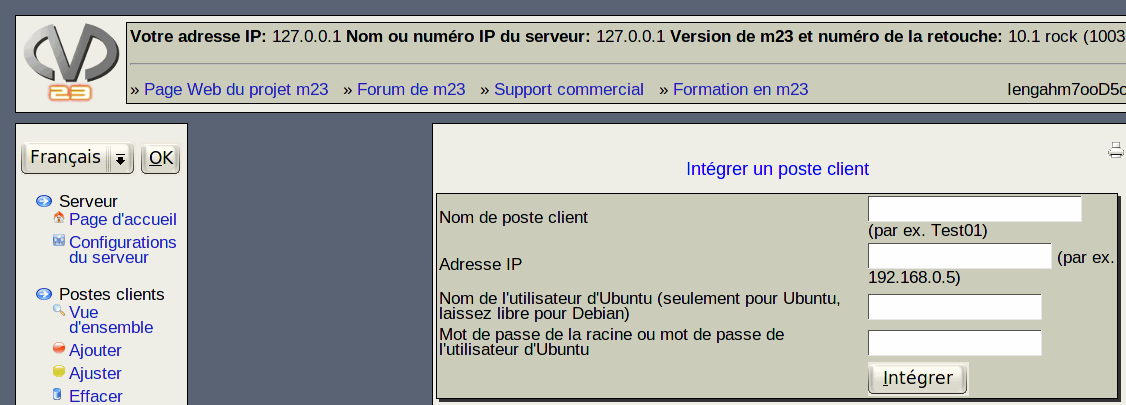
\includegraphics[scale=0.4]{/mdk/doc/manual/screenshots/en/client_assimilate.png} \\
After the assimilation over this dialog you can administrate existing Debian systems with m23. The client must be started up completely and reachable over the network for smooth assimilation. Now you have to enter only three values:\\
\begin{itemize}
\item \textbf{Client name}: This is the name the client should be known by the m23 server. It is advised, but not required to enter the hostname of the client.\\
\item \textbf{IP Address}: This is the (temporary) IP address of the client\\
\item \textbf{Name of the Ubuntu user (only for assimilating Ubuntu systems. Keep empty for Debian)}: Enter here a username that is known to the system and that is allowed to log in via SSH and execute commands via sudo as root with the same password. This is only needed on computers installed with Ubuntu or with disabled root logins.\\
\item \textbf{Root password or password of the Ubuntu user}: This is the current root password of the client or the user password on Ubuntu systems. You can leave empty this field too if you prefer manual intergration.\\
\end{itemize}
Click on \textit{"Assimilate"} afterwards. The assimilation is done in the background.\\
\subsection{Hint}
For automatic assimilation a running SSH daemon that allows logging in as "root" is required on client side. The programm "wget" and the package "coreutils" have to be installed too. And at last it is required that packages can be installed via APT and downloaded from the internet.\\
\subsection{Manual assimilation}
You can start the assimilation by hand if there is no SSH daemon running on the client. Execute the following commands as root in a console on the client (replace "serverIP" with the IP of your m23 server):\\
\begin{verbatim}
cd /tmp; wget http://$\langle$serverIP$\rangle$/work.php -O work.php; sh work.php
\end{verbatim}
\subsection{Hint for the assimilation of an Ubuntu system}
Ubuntu systems can be assimilated normally with "manual assimilation" only, because there is no running SSH daemon . Please start a root console on the Ubuntu system and continue with the hint "Manual assimilation".\\
